For stars with $B-V\le0.58$ (corresponding to an F9.5 spectral type and approximate main-sequence mass of $1.1M_{\odot}$), we apply additional constraints on their ages based on stellar lifetimes and their CMD positions \rev{(e.g. \citealt{2013ApJ...776....4N, 2019AJ....158...13N})}. Using this technique, we also produce age posteriors for stars too massive for Li, $R^{'}_{HK}$, or gyrochronology. CMD age posteriors are especially useful in cases where we can only derive a lower limit on the age from a lithium equivalent width upper limit because the stellar lifetime can be used to constrain the upper bound on the age (e.g. late F stars). To calculate CMD position-based age posteriors, we follow the method from \cite{2019AJ....158...13N}, which uses a Bayesian approach to \rev{compute ages from stellar models and optical photometry. For each star, MCMC is used to explore the 5-dimensional parameter space in stellar mass, age, metallicity, initial rotation, inclination of the rotation axis, and parallax. We use the same priors on these parameters as in \cite{2019AJ....158...13N}, and a Gaussian likelihood for the $Gaia$ $G_B$, $G$, and $G_R$ catalog photometry and errors. The model predictions at each MCMC step are generated, as in \cite{2019AJ....158...13N}, from a combination of MESA \citep{2011ApJS..192....3P} evolutionary models with ATLAS9 model atmospheres \citep{2004A&A...419..725C}.} As in \cite{2019AJ....158...13N}, for stars with $B-V\leq0.27$, we include a prior based on the metallicity distribution of stars $<1$ Gyr from \cite{2011A&A...530A.138C}.

For \rev{55} stars more than one age tracer is available, and we improve our constraints by taking the product of each age posterior for a given star. In Table \ref{tab:general} we present our full 166-star sample, including basic properties and \rev{final median ages and $68\%$ and $95\%$ confidence intervals for each star}. Figure \ref{bmv_age} shows the age posteriors for the sample as a function of $B-V$.




\begin{figure*}[hb!]
\centering
 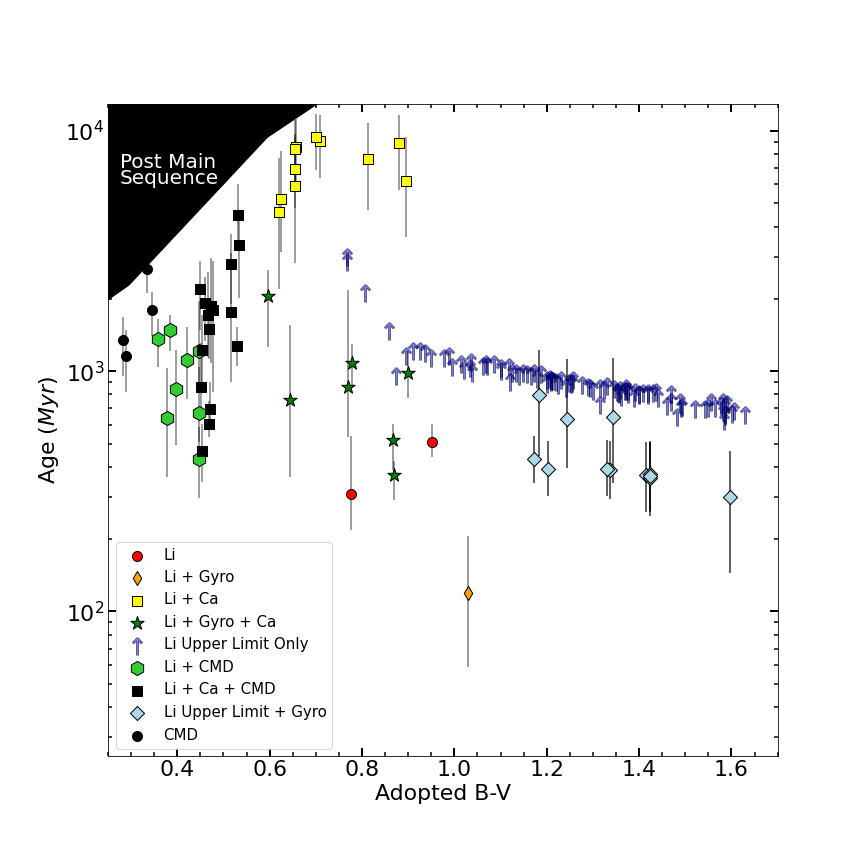
\includegraphics[scale = 0.35]{age_bmv.png}

 \caption{The medians and $68\%$ confidence intervals for our derived age posteriors for the full sample of 166 stars, as a function of $B-V$. The symbol and color of each star represent which age tracer (or tracers) was used to derive the age posterior. The error bars represent the $68\%$ confidence intervals.}
 \label{bmv_age}
\end{figure*}




{\setlength{\tabcolsep}{4pt}\begin{longrotatetable}
\begin{deluxetable}{|c|c|c|c|c|c|c|c|c|c|c|c|}
%\begin{longtable}{|c|c|c|c|c|c|c|c|c|c|c|}
\centering
\tabletypesize{\scriptsize}
\tablecaption{Our complete sample of accelerating stars with age posteriors and age tracers used. Ages come from a combination of lithium (Li), lithium upper limits (Li UL),\\ calcium emission (R'HK), rotation periods (Gyro), and CMD positions (CMD). Age posteriors are either presented as a median with $68\%$ and $95\%$ confidence intervals or as $68\%$,\\ $95\%$ and $99.7\%$ lower limits.}
%\hline
\tablehead{
\colhead{}  & \colhead{}  &\colhead{}   & \colhead{}  & \colhead{}  & \colhead{}  & \colhead{}  & \colhead{}    & \colhead{Median Age}  & \colhead{$68\%$ CI}   & \colhead{$95\%$ CI} \\
\colhead{Target}  & \colhead{R.A.}  &\colhead{Dec.}   & \colhead{G}  & \colhead{Adopted}   & \colhead{Simbad} & \colhead{Dist}  & \colhead{Tracers}  & \colhead{ or $68\%$ LL}  & \colhead{or $95\%$ LL}   & \colhead{or $99.7\%$ LL} \\
\colhead{} & \colhead{}  & \colhead{} & \colhead{mag}  & \colhead{$B-V$}  &\colhead{Spec. Type}   & \colhead{(pc)}  &\colhead{} & \colhead{(Myr)} & \colhead{(Myr)} & \colhead{(Myr)} }
%\hline

\startdata
HIP 143 &  00 01 49.35 &  +21 27 45.01 &  $ 9.9811 \pm 0.0002 $ &  $ 1.033 \pm 0.019 $ &  K3 & $ 43.4 \pm  0.59 $&  Li UL & $\ge 4442.08 $ & $\ge 1034.76 $ & $\ge 484.61 $ \\
HIP 669 &  00 08 16.36 &  -14 49 28.16 &  $ 6.8956 \pm 0.0002 $ &  $ 0.624 \pm 0.015 $ &   G1V & $ 27.31 \pm  0.02 $&  Li, R'HK &  5234.81 &  3132.71-8290.74 &  1783.08-11668.88 \\
HIP 1068 &  00 13 15.83 &  +69 19 36.76 &  $ 12.0476 \pm 0.0015 $ &  $ 1.315 \pm 0.1 $ &   M4 & $ 20.52 \pm  0.05 $&  Li UL & $\ge 4217.04 $ & $\ge 720.14 $ & $\ge 138.08 $ \\
HIP 1412 &  00 17 40.90 &  -08 40 56.14 &  $ 10.2711 \pm 0.0006 $ &  $ 1.414 \pm 0.005 $ &  K7V & $ 32.05 \pm  0.09 $&  Li UL, Gyro &  367.99 &  258.82-508.19 &  148.22-612.04 \\
HIP 1539 &  00 19 12.39 &  -03 03 13.01 &  $ 10.2808 \pm 0.0004 $ &  $ 1.375 \pm 0.005 $ &   K5V & $ 31.19 \pm  0.02 $&  Li UL & $\ge 4294.84 $ & $\ge 828.91 $ & $\ge 280.46 $ \\
HIP 1771 &  00 22 25.19 &  +06 40 03.16 &  $ 10.6176 \pm 0.0005 $ &  $ 1.489 \pm 0.1 $ &   K7V & $ 43.88 \pm  0.09 $&  Li UL & $\ge 4234.75 $ & $\ge 744.83 $ & $\ge 164 $ \\
HIP 2426 &  00 30 55.58 &  +73 22 14.89 &  $ 10.0247 \pm 0.0002 $ &  $ 1.359 \pm 0.02 $ &   K & $ 29.48 \pm  0.01 $&  Li UL & $\ge 4298.94 $ & $\ge 834.64 $ & $\ge 285.77 $ \\
HIP 2843 &  00 36 01.85 &  -05 34 14.58 &  $ 6.6114 \pm 0.0002 $ &  $ 0.466 \pm 0.007 $ &   F6V & $ 44.84 \pm  0.06 $&  Li UL, R'HK, CMD &  1715.26 &  1150.23-2585.26 &  808.98-3587.63 \\
HIP 3008 &  00 38 15.29 &  +52 19 55.52 &  $ 9.8115 \pm 0.0003 $ &  $ 1.424 \pm 0.02 $ &   M0.0V & $ 23.02 \pm  0.01 $&  Li UL, Gyro &  360.24 &  250.15-502.94 &  128.65-609.82 \\
HIP 3293 &  00 42 01.42 &  +40 41 17.71 &  $ 6.9164 \pm 0.0003 $ &  $ 0.452 \pm 0.009 $ &   F5 & $ 49.58 \pm  0.07 $&  Li, R'HK, CMD &  862.22 &  651.1-1311.35 &  521.75-2077.47 \\
HIP 3633 &  00 46 34.04 &  +14 19 31.61 &  $ 9.6005 \pm 0.0001 $ &  $ 0.814 \pm 0.061 $ &   K3V & $ 46.51 \pm  0.21 $&  Li UL, R'HK &  7664.88 &  4696.93-10795.26 &  2383.87-12584.18 \\
HIP 3724 &  00 47 48.47 &  +06 01 54.92 &  $ 10.963 \pm 0.0004 $ &  $ 1.4 \pm 0.02 $ &   M0.0V & $ 40.62 \pm  0.05 $&  Li UL & $\ge 4277.49 $ & $\ge 804.65 $ & $\ge 255.04 $ \\
HIP 4024 &  00 51 34.56 &  -14 53 26.46 &  $ 9.4072 \pm 0.0002 $ &  $ 1.069 \pm 0.009 $ &   K3.5IV-V & $ 43.46 \pm  0.15 $&  Li UL & $\ge 4471.25 $ & $\ge 1075.56 $ & $\ge 530.93 $ \\
HIP 5319 &  01 08 01.34 &  +32 00 43.66 &  $ 6.1346 \pm 0.0003 $ &  $ 0.398 \pm 0.01 $ &  F5IV & $ 42.9 \pm  0.06 $&  Li UL, CMD &  843.22 &  495.26-1230.45 &  219.62-1644.67 \\
HIP 5763 &  01 13 58.86 &  +16 29 40.26 &  $ 9.3939 \pm 0.0002 $ &  $ 1.22 \pm 0.015 $ & K6V & $ 32.01 \pm  0.03 $&  Li UL & $\ge 4348.13 $ & $\ge 903.42 $ & $\ge 352.3 $ \\
HIP 6776 &  01 27 06.32 &  +34 22 39.18 &  $ 6.1623 \pm 0.0003 $ &  $ 0.453 \pm 0.007 $ &   F7IVsv & $ 42.05 \pm  0.05 $&  Li UL, R'HK, CMD &  1220.64 &  830.65-1719.17 &  617.88-2140.42 \\
HIP 6796 &  01 27 27.60 &  +23 14 40.42 &  $ 9.4186 \pm 0.0004 $ &  $ 1.157 \pm 0.074 $ &  K7V & $ 37.17 \pm  0.04 $&  Li UL & $\ge 4400.69 $ & $\ge 976.89 $ & $\ge 409.71 $ \\
HIP 6833 &  01 27 55.56 &  -01 59 29.35 &  $ 8.4502 \pm 0.0002 $ &  $ 0.656 \pm 0.002 $ &  G5V & $ 48.1 \pm  0.06 $&  Li, R'HK &  6929.95 &  4767.61-9685.66 &  2971.34-12173.29 \\
HIP 6943 &  01 29 26.45 &  +42 16 54.85 &  $ 7.078 \pm 0.0003 $ &  $ 0.453 \pm 0.011 $ &   F5 & $ 48.19 \pm  0.06 $&  Li, R'HK, CMD &  466.38 &  344.95-600.94 &  208.59-1059.12 \\
HIP 7287 &  01 33 53.62 &  +27 14 08.74 &  $ 10.5178 \pm 0.0002 $ &  $ 1.2 \pm 0.02 $ &   K5 & $ 48.57 \pm  0.22 $&  Li UL & $\ge 4334.42 $ & $\ge 884.25 $ & $\ge 332.72 $ \\
HIP 8653 &  01 51 31.19 &  -07 44 23.57 &  $ 8.4607 \pm 0.0003 $ &  $ 0.644 \pm 0.019 $ &   G5V & $ 47.89 \pm  1.09 $&  Li, Gyro, R'HK &  759.94 &  364.45-1561.09 &  185.93-2455.98 \\
HIP 9067 &  01 56 43.73 &  +29 48 39.04 &  $ 10.8658 \pm 0.0003 $ &  $ 1.47 \pm 0.1 $ &  K5V & $ 47.3 \pm  0.03 $&  Li UL & $\ge 4275.7 $ & $\ge 801.85 $ & $\ge 231.94 $ \\
HIP 9989 &  02 08 40.08 &  -00 21 35.61 &  $ 10.4039 \pm 0.0003 $ &  $ 1.248 \pm 0.002 $ &   K5V & $ 39.45 \pm  0.03 $&  Li UL & $\ge 4340.02 $ & $\ge 892.08 $ & $\ge 341.68 $ \\
HIP 10050 &  02 09 23.11 &  +17 13 27.11 &  $ 6.2937 \pm 0.0003 $ &  $ 0.471 \pm 0.001 $ &   F5V & $ 36.32 \pm  0.04 $&  Li, R'HK, CMD &  694.63 &  612.9-897.62 &  509.72-1344.86 \\
HIP 10532 &  02 15 41.72 &  -09 00 47.23 &  $ 8.877 \pm 0.0002 $ &  $ 0.88 \pm 0.033 $ &   K0V & $ 44.19 \pm  0.03 $&  Li UL, R'HK &  8922.3 &  5685.95-11625.28 &  2863.63-12794.61 \\
HIP 11090 &  02 22 50.30 &  +41 23 46.65 &  $ 5.7433 \pm 0.0009 $ &  $ 0.289 \pm 0.006 $ &  F0III-IV & $ 48.33 \pm  0.14 $&  CMD &  1155.1 &  820.23-1479.52 &  520.53-1744.73 \\
HIP 11815 &  02 32 23.18 &  +03 22 57.48 &  $ 11.2101 \pm 0.0014 $ &  $ 1.357 \pm 0.02 $ &  K5 & $ 49.26 \pm  0.05 $&  Li UL & $\ge 4276.65 $ & $\ge 803.47 $ & $\ge 253.41 $ \\
HIP 12837 &  02 45 01.09 &  -22 09 59.51 &  $ 7.0178 \pm 0.0002 $ &  $ 0.517 \pm 0.008 $ &   F7V & $ 38.9 \pm  0.03 $&  Li, R'HK, CMD &  1771.7 &  899.96-3111.02 &  386.64-4669.22 \\
HIP 13681 &  02 56 14.10 &  -11 50 49.84 &  $ 9.8618 \pm 0.0003 $ &  $ 1.062 \pm 0.015 $ &   -- & $ 47.51 \pm  0.04 $&  Li UL & $\ge 4456.4 $ & $\ge 1054.8 $ & $\ge 509.53 $ \\
HIP 13782 &  02 57 23.76 &  -23 51 43.79 &  $ 5.399 \pm 0.0005 $ &  $ 0.238 \pm 0.003 $ &   A5IV/V & $ 48.69 \pm  0.15 $&  CMD &  757.31 &  595.43-917.22 &  443.02-1075.26 \\
HIP 15211 &  03 16 05.89 &  -05 51 15.85 &  $ 9.9066 \pm 0.0002 $ &  $ 0.936 \pm 0.007 $ &  K3 & $ 49.29 \pm  0.04 $&  Li UL & $\ge 4551.82 $ & $\ge 1187.49 $ & $\ge 609.82 $ \\
HIP 16247 &  03 29 22.87 &  -24 06 03.09 &  $ 8.8107 \pm 0.0005 $ &  $ 1.02 \pm 0.037 $ &  K3VkFe+0.4 & $ 31.08 \pm  0.02 $&  Li UL & $\ge 4428.57 $ & $\ge 1015.84 $ & $\ge 461.81 $ \\
HIP 16709 &  03 34 59.64 &  +34 36 39.51 &  $ 10.3002 \pm 0.0004 $ &  $ 1.225 \pm 0.02 $ &   M0 & $ 41.1 \pm  0.65 $&  Li UL & $\ge 4331.28 $ & $\ge 879.86 $ & $\ge 328.75 $ \\
HIP 17118 &  03 39 58.81 &  +63 52 13.47 &  $ 6.7675 \pm 0.0002 $ &  $ 0.478 \pm 0.023 $ &   F5 & $ 42.81 \pm  0.03 $&  Li, R'HK, CMD &  1790.5 &  818.76-2885.78 &  405.89-3903.25 \\
HIP 17213 &  03 41 13.71 &  +75 23 56.51 &  $ 9.6211 \pm 0.0006 $ &  $ 1.1 \pm 0.015 $ &   K0 & $ 43.63 \pm  0.08 $&  Li UL & $\ge 4420.43 $ & $\ge 1004.51 $ & $\ge 453.14 $ \\
HIP 18527 &  03 57 43.92 &  -20 16 04.05 &  $ 8.6088 \pm 0.0004 $ &  $ 0.899 \pm 0.021 $ &   K2VkFe-0.5 & $ 37.38 \pm  0.03 $&  Li UL, Gyro, R'HK &  981.67 &  770.11-1216.88 &  619.34-1469.49 \\
HIP 19739 &  04 13 55.87 &  +82 55 06.98 &  $ 10.1025 \pm 0.0005 $ &  $ 1.424 \pm 0.02 $ &   M0.0V & $ 36.94 \pm  0.17 $&  Li UL, Gyro &  372.38 &  265.37-510.32 &  199.63-612.75 \\
HIP 19912 &  04 16 18.56 &  +08 43 09.96 &  $ 9.4283 \pm 0.0002 $ &  $ 1.148 \pm 0.002 $ &   K7V & $ 38.96 \pm  0.26 $&  Li UL & $\ge 4408.38 $ & $\ge 987.64 $ & $\ge 433.87 $ \\
HIP 20419 &  04 22 25.69 &  +11 18 20.56 &  $ 9.3585 \pm 0.0004 $ &  $ 1.183 \pm 0.005 $ &   K2 & $ 44.05 \pm  0.48 $&  Li UL, Gyro &  797.7 &  444.12-1230.22 &  313.95-1599.99 \\
HIP 20648 &  04 25 29.38 &  +17 55 40.46 &  $ 4.2957 \pm 0.001 $ &  $ 0.049 \pm 0.007 $ &   A2IV-Vs & $ 47.42 \pm  0.31 $&  CMD &  602.61 &  530.07-670.92 &  456.89-742.38 \\
HIP 21066 &  04 30 57.17 &  +10 45 06.36 &  $ 6.9211 \pm 0.0002 $ &  $ 0.472 \pm 0.013 $ &   F7V & $ 46.51 \pm  0.06 $&  Li UL, R'HK, CMD &  1864.19 &  1085.7-2959.28 &  650.55-3268.37 \\
HIP 21152 &  04 32 04.80 &  +05 24 36.14 &  $ 6.2678 \pm 0.0002 $ &  $ 0.42 \pm 0.014 $ &   F5V & $ 43.27 \pm  0.05 $&  Li UL, CMD &  1116.14 &  765.3-1521.58 &  423.86-1861.12 \\
HIP 22361 &  04 48 50.35 &  +75 56 28.39 &  $ 5.8984 \pm 0.0004 $ &  $ 0.283 \pm 0.004 $ &   A9IV & $ 47.6 \pm  0.06 $&  CMD &  1350.34 &  959.72-1684.76 &  602.75-1979.1 \\
HIP 23208 &  04 59 38.25 &  -10 59 02.26 &  $ 9.3009 \pm 0.0004 $ &  $ 1.18 \pm 0.006 $ &  K5Vk & $ 34.82 \pm  0.05 $&  Li UL & $\ge 4365.63 $ & $\ge 927.89 $ & $\ge 376.02 $ \\
HIP 24017 &  05 09 44.50 &  +64 55 10.16 &  $ 6.2661 \pm 0.0002 $ &  $ 0.448 \pm 0.004 $ &   F3V & $ 39.09 \pm  0.03 $&  Li UL, CMD &  1216.34 &  828.62-1964.68 &  633.89-2692.15 \\
HIP 24177 &  05 11 29.73 &  +10 07 15.66 &  $ 11.156 \pm 0.0005 $ &  $ 1.461 \pm 0.005 $ &  M0V & $ 44.19 \pm  0.18 $&  Li UL & $\ge 4216.67 $ & $\ge 719.62 $ & $\ge 159.14 $ \\
HIP 24292 &  05 12 47.95 &  +16 18 25.43 &  $ 10.1675 \pm 0.0003 $ &  $ 1.23 \pm 0.015 $ &  K7V & $ 44.01 \pm  0.03 $&  Li UL & $\ge 4357.55 $ & $\ge 916.6 $ & $\ge 365.54 $ \\
HIP 24457 &  05 14 49.83 &  +00 42 31.67 &  $ 9.4575 \pm 0.0002 $ &  $ 1.118 \pm 0.005 $ &  K5V & $ 39.6 \pm  0.02 $&  Li UL & $\ge 4445.1 $ & $\ge 1038.96 $ & $\ge 482.73 $ \\
HIP 25606 &  05 28 14.72 &  -20 45 33.99 &  $ 2.6272 \pm 0.0015 $ &  $ 0.807 \pm 0.027 $ &  G5II-IIIa & $ 47.92 \pm  0.47 $&  Li UL & $\ge 5405.2 $ & $\ge 2111.49 $ & $\ge 1021.51 $ \\
HIP 27021 &  05 43 52.79 &  -21 16 47.04 &  $ 6.9723 \pm 0.0001 $ &  $ 0.531 \pm 0.006 $ &   F8/G0V & $ 43.2 \pm  0.03 $&  Li, R'HK, CMD &  4464.59 &  3159.78-5991.22 &  2077.47-7143.76 \\
HIP 28823 &  06 05 03.38 &  +42 58 53.88 &  $ 5.8206 \pm 0.0006 $ &  $ 0.358 \pm 0.005 $ & F3V & $ 49.78 \pm  0.22 $&  Li UL, CMD &  1360.86 &  1038.87-1642.63 &  703.98-1867.14 \\
HIP 29208 &  06 09 35.91 &  +05 40 08.05 &  $ 8.194 \pm 0.0002 $ &  $ 0.895 \pm 0.022 $ &   G0 & $ 30.19 \pm  0.02 $&  Li UL & $\ge 4526.8 $ & $\ge 1152.02 $ & $\ge 568.66 $ \\
HIP 33282 &  06 55 23.46 &  +44 25 19.30 &  $ 10.7232 \pm 0.0004 $ &  $ 1.344 \pm 0.035 $ &  K6V & $ 48.22 \pm  0.03 $&  Li UL, Gyro &  647.7 &  341.31-1139.51 &  248.03-1546.97 \\
HIP 33368 &  06 56 22.10 &  +46 59 26.75 &  $ 10.4419 \pm 0.0005 $ &  $ 1.346 \pm 0.1 $ &  K7V & $ 47.17 \pm  0.06 $&  Li UL & $\ge 4308.04 $ & $\ge 847.34 $ & $\ge 288 $ \\
HIP 34804 &  07 12 17.20 &  +59 15 51.95 &  $ 10.2697 \pm 0.0003 $ &  $ 1.591 \pm 0.082 $ & K4 & $ 38.93 \pm  0.7 $&  Li UL & $\ge 4224.76 $ & $\ge 730.29 $ & $\ge 157.52 $ \\
HIP 36081 &  07 26 03.61 &  -15 39 57.28 &  $ 6.7409 \pm 0.0002 $ &  $ 0.62 \pm 0.005 $ &  G1/2V & $ 49.68 \pm  0.46 $&  Li, R'HK &  4585.75 &  2189.37-7747.86 &  1010.09-11446.52 \\
HIP 37267 &  07 39 10.33 &  +29 54 32.16 &  $ 10.4391 \pm 0.0006 $ &  $ 1.277 \pm 0.022 $ &   K5V & $ 48.9 \pm  0.03 $&  Li UL & $\ge 4328.24 $ & $\ge 875.61 $ & $\ge 325.41 $ \\
HIP 40518 &  08 16 23.06 &  -17 22 03.83 &  $ 10.0726 \pm 0.0003 $ &  $ 1.134 \pm 0.004 $ &  -- & $ 46.43 \pm  0.6 $&  Li UL & $\ge 4406.56 $ & $\ge 985.1 $ & $\ge 430.98 $ \\
HIP 41274 &  08 25 14.08 &  -07 10 12.85 &  $ 7.0892 \pm 0.0006 $ &  $ 0.952 \pm 0.011 $ &  K0V & $ 49.14 \pm  0.07 $&  Li &  505.8 &  439.44-602.43 &  335.92-820.22 \\
HIP 41277 &  08 25 16.90 &  +04 15 12.72 &  $ 9.9158 \pm 0.002 $ &  $ 1.03 \pm 0.015 $ &  K8V & $ 41.68 \pm  0.08 $&  Li, Gyro &  119.62 &  58.63-206.48 &  17.47-300.01 \\
HIP 41319 &  08 25 49.87 &  +17 02 46.57 &  $ 5.9986 \pm 0.0003 $ &  $ 0.448 \pm 0.005 $ &  F5IIIm? & $ 45.5 \pm  0.07 $&  Li, CMD &  668.73 &  509.36-1040.76 &  400.75-1505.21 \\
HIP 42231 &  08 36 37.96 &  +39 02 13.55 &  $ 11.2749 \pm 0.0003 $ &  $ 1.241 \pm 0.015 $ &   -- & $ 43.88 \pm  0.15 $&  Li UL & $\ge 4308.4 $ & $\ge 847.87 $ & $\ge 296.87 $ \\
HIP 42343 &  08 37 57.55 &  -08 52 53.72 &  $ 6.9078 \pm 0.0002 $ &  $ 0.516 \pm 0.001 $ &   F6V & $ 48.73 \pm  0.05 $&  Li, R'HK, CMD &  2791.29 &  1896.43-3724.4 &  1184.85-4152.26 \\
HIP 42507 &  08 40 00.26 &  -06 28 33.06 &  $ 9.2424 \pm 0.0003 $ &  $ 1.361 \pm 0.001 $ &  K6V & $ 25.46 \pm  0.09 $&  Li UL & $\ge 4259.1 $ & $\ge 778.95 $ & $\ge 226.84 $ \\
HIP 43745 &  08 54 35.72 &  +63 45 29.74 &  $ 10.4509 \pm 0.0002 $ &  $ 1.423 \pm 0.02 $ &   K5V & $ 34.26 \pm  0.02 $&  Li UL, Gyro &  366.55 &  260.53-505.31 &  168.77-610.43 \\
HIP 44162 &  08 59 39.91 &  -19 12 28.95 &  $ 6.0845 \pm 0.0003 $ &  $ 0.461 \pm 0.005 $ &   F5V & $ 40.24 \pm  0.13 $&  Li UL, R'HK, CMD &  1925.01 &  1340.03-2478.25 &  901.96-3477.51 \\
HIP 44953 &  09 09 30.16 &  -00 23 54.35 &  $ 8.4254 \pm 0.0002 $ &  $ 0.767 \pm 0.002 $ &   G8V & $ 34.95 \pm  0.03 $&  Li UL & $\ge 5993.75 $ & $\ge 2846.19 $ & $\ge 1323.58 $ \\
HIP 45621 &  09 17 55.38 &  -03 23 14.09 &  $ 7.5442 \pm 0.0003 $ &  $ 0.869 \pm 0.013 $ &   K1/2V & $ 32.28 \pm  0.04 $&  Li, Gyro, R'HK &  371.47 &  291.48-423.05 &  144.29-489.92 \\
HIP 45731 &  09 19 22.86 &  +62 03 16.89 &  $ 10.5142 \pm 0.0006 $ &  $ 1.586 \pm 0.02 $ &   M1.0Ve & $ 37.94 \pm  0.03 $&  Li UL & $\ge 4167.6 $ & $\ge 650.87 $ & $\ge 91.63 $ \\
HIP 46385 &  09 27 30.56 &  +50 39 12.45 &  $ 10.9763 \pm 0.0005 $ &  $ 1.586 \pm 0.1 $ &   M2.5V & $ 31.16 \pm  0.05 $&  Li UL & $\ge 4175.04 $ & $\ge 661.4 $ & $\ge 92.44 $ \\
HIP 47013 &  09 34 53.52 &  +72 12 20.44 &  $ 5.6501 \pm 0.0005 $ &  $ 0.53 \pm 0.003 $ &   F7V & $ 49.6 \pm  0.08 $&  Li UL, R'HK, CMD &  1275.94 &  1054.99-1523.22 &  861.32-1758.82 \\
HIP 47261 &  09 37 58.33 &  +22 31 23.15 &  $ 9.4588 \pm 0.0003 $ &  $ 1.21 \pm 0.015 $ &   K4V & $ 30.89 \pm  0.02 $&  Li UL & $\ge 4351.49 $ & $\ge 908.11 $ & $\ge 356.79 $ \\
HIP 47300 &  09 38 21.77 &  +40 14 23.25 &  $ 5.237 \pm 0.0007 $ &  $ 0.223 \pm 0.004 $ &   F0V & $ 38.49 \pm  0.12 $&  CMD &  718.62 &  500.33-934.73 &  298.93-1134.22 \\
HIP 47387 &  09 39 14.59 &  +66 50 58.14 &  $ 9.6883 \pm 0.0002 $ &  $ 1.07 \pm 0.047 $ &   K2 & $ 41.63 \pm  0.54 $&  Li UL & $\ge 4450.55 $ & $\ge 1046.57 $ & $\ge 489.6 $ \\
HIP 47539 &  09 41 31.44 &  -06 23 35.83 &  $ 11.2695 \pm 0.0004 $ &  $ 1.353 \pm 0.011 $ & -- & $ 44.42 \pm  0.37 $&  Li UL & $\ge 4288.12 $ & $\ge 819.51 $ & $\ge 270.07 $ \\
HIP 47741 &  09 43 55.61 &  +26 58 08.40 &  $ 10.8486 \pm 0.0004 $ &  $ 1.542 \pm 0.039 $  & M3.5V & $ 14.37 \pm  0.01 $&  Li UL & $\ge 4202.01 $ & $\ge 698.97 $ & $\ge 130.85 $ \\
HIP 48165 &  09 49 03.16 &  +07 49 08.68 &  $ 9.5048 \pm 0.0002 $ &  $ 0.925 \pm 0.015 $  & G5 & $ 45.77 \pm  0.48 $&  Li UL & $\ge 4574.64 $ & $\ge 1219.3 $ & $\ge 638.59 $ \\
HIP 48629 &  09 54 59.84 &  +40 23 07.28 &  $ 10.7594 \pm 0.0002 $ &  $ 1.581 \pm 0.197 $  & K5V & $ 37.37 \pm  0.04 $&  Li UL & $\ge 4234.47 $ & $\ge 744.26 $ & $\ge 152.31 $ \\
HIP 49046 &  10 00 26.71 &  +27 16 01.61 &  $ 10.5279 \pm 0.0002 $ &  $ 1.372 \pm 0.015 $  & M0.5V & $ 36.01 \pm  0.02 $&  Li UL & $\ge 4292.26 $ & $\ge 825.31 $ & $\ge 276.52 $ \\
HIP 49526 &  10 06 43.80 &  +41 42 52.65 &  $ 10.5229 \pm 0.0003 $ &  $ 1.492 \pm 0.02 $  & M1.0V & $ 22.28 \pm  0.02 $&  Li UL & $\ge 4210.41 $ & $\ge 710.86 $ & $\ge 147.69 $ \\
HIP 49577 &  10 07 13.74 &  -14 18 16.54 &  $ 9.6168 \pm 0.0004 $ &  $ 1.331 \pm 0.014 $ & K5V & $ 39.53 \pm  0.64 $&  Li UL & $\ge 4322.44 $ & $\ge 867.5 $ & $\ge 318.63 $ \\
HIP 49910 &  10 11 23.70 &  -01 39 44.69 &  $ 11.1457 \pm 0.0004 $ &  $ 1.391 \pm 0.023 $ &   -- & $ 46.55 \pm  0.04 $&  Li UL & $\ge 4286.95 $ & $\ge 817.89 $ & $\ge 268.72 $ \\
HIP 51208 &  10 27 34.85 &  +12 58 48.14 &  $ 10.2039 \pm 0.0003 $ &  $ 1.2 \pm 0.015 $ &  K4V & $ 46.38 \pm  0.46 $&  Li UL & $\ge 4361.89 $ & $\ge 922.66 $ & $\ge 371.01 $ \\
HIP 52339 &  10 41 48.44 &  +12 06 31.90 &  $ 10.9365 \pm 0.0003 $ &  $ 1.42 \pm 0.015 $  & K7V & $ 37.04 \pm  0.03 $&  Li UL & $\ge 4281.04 $ & $\ge 809.62 $ & $\ge 260.19 $ \\
HIP 53175 &  10 52 39.61 &  +00 29 01.95 &  $ 10.1771 \pm 0.0004 $ &  $ 1.293 \pm 0.005 $  & K4V & $ 39.35 \pm  0.03 $&  Li UL & $\ge 4312.99 $ & $\ge 854.28 $ & $\ge 304.58 $ \\
HIP 53869 &  11 01 16.35 &  +29 35 27.47 &  $ 9.4421 \pm 0.0003 $ &  $ 0.868 \pm 0.045 $  & K3V & $ 49.58 \pm  0.06 $&  Li UL, Gyro, R'HK &  515.87 &  388.61-604.35 &  245.7-648.74 \\
HIP 54094 &  11 04 07.15 &  +53 22 55.47 &  $ 9.7081 \pm 0.0001 $ &  $ 1.1 \pm 0.02 $ &   -- & $ 46.51 \pm  0.03 $&  Li UL & $\ge 4441.41 $ & $\ge 1033.83 $ & $\ge 481.2 $ \\
HIP 54199 &  11 05 16.57 &  +65 48 49.51 &  $ 8.2868 \pm 0.0001 $ &  $ 0.874 \pm 0.016 $  & G5 & $ 39.08 \pm  0.45 $&  Li UL & $\ge 4383.16 $ & $\ge 952.11 $ & $\ge 383.88 $ \\
HIP 55192 &  11 18 00.48 &  +35 26 41.81 &  $ 8.0635 \pm 0.0003 $ &  $ 0.776 \pm 0.015 $ &   G5 & $ 39.7 \pm  0.17 $&  Li &  308.96 &  218.51-539.13 &  66.28-1459.69 \\
HIP 55409 &  11 20 51.76 &  -23 13 02.42 &  $ 7.8415 \pm 0.0002 $ &  $ 0.658 \pm 0.003 $ &   G3/5V & $ 42.16 \pm  0.04 $&  Li UL, R'HK &  8592.32 &  5708.12-11271.52 &  3349.2-12735.77 \\
HIP 57361 &  11 45 34.44 &  -20 21 12.38 &  $ 10.8203 \pm 0.0004 $ &  $ 1.482 \pm 0.015 $ &   M2.5V & $ 19.2 \pm  0.06 $&  Li UL & $\ge 4164.34 $ & $\ge 646.46 $ & $\ge 85.43 $ \\
HIP 57571 &  11 48 01.50 &  +71 21 28.14 &  $ 10.754 \pm 0.0002 $ &  $ 1.369 \pm 0.02 $ &  -- & $ 45.93 \pm  0.35 $&  Li UL & $\ge 4295.72 $ & $\ge 830.14 $ & $\ge 281.31 $ \\
HIP 57645 &  11 49 13.15 &  -20 20 34.67 &  $ 8.9933 \pm 0.0002 $ &  $ 0.895 \pm 0.015 $ &  G3V & $ 38.12 \pm  0.03 $&  Li UL, R'HK &  6204.18 &  3637.04-9422.01 &  1781.04-12308.42 \\
HIP 57984 &  11 53 37.20 &  +49 36 01.07 &  $ 10.5512 \pm 0.0002 $ &  $ 1.316 \pm 0.015 $ &  K5 & $ 45.0 \pm  0.15 $&  Li UL & $\ge 4310.95 $ & $\ge 851.43 $ & $\ge 302.07 $ \\
HIP 59000 &  12 05 50.66 &  -18 52 30.92 &  $ 9.3933 \pm 0.0007 $ &  $ 1.336 \pm 0.014 $ &  K5V & $ 23.06 \pm  0.05 $&  Li UL, Gyro &  388.45 &  293.22-514.42 &  219.44-613.01 \\
HIP 59198 &  12 08 22.20 &  -00 28 57.36 &  $ 10.5473 \pm 0.0004 $ &  $ 1.409 \pm 0.015 $ &  K4V & $ 29.13 \pm  0.08 $&  Li UL & $\ge 4283.83 $ & $\ge 813.52 $ & $\ge 264.26 $ \\
HIP 59199 &  12 08 24.81 &  -24 43 43.95 &  $ 3.9466 \pm 0.0013 $ &  $ 0.334 \pm 0.015 $ &   F1V & $ 14.98 \pm  0.04 $&  CMD &  2665.78 &  2119.54-3334.23 &  1360.6-3849.28 \\
HIP 59247 &  12 09 13.08 &  +19 28 03.61 &  $ 10.4409 \pm 0.0003 $ &  $ 1.29 \pm 0.015 $ &   K7V & $ 41.84 \pm  0.03 $&  Li UL & $\ge 4317.08 $ & $\ge 860.01 $ & $\ge 310.2 $ \\
HIP 59767 &  12 15 20.27 &  +87 42 00.42 &  $ 6.1886 \pm 0.0008 $ &  $ 0.346 \pm 0.011 $ &   F1IV & $ 48.38 \pm  0.05 $&  CMD &  1793.47 &  1401.11-2138.93 &  945.46-2464.7 \\
HIP 59905 &  12 17 15.20 &  -07 48 43.93 &  $ 10.0396 \pm 0.0003 $ &  $ 1.125 \pm 0.015 $ &   K4V & $ 47.71 \pm  0.05 $&  Li UL & $\ge 4406.67 $ & $\ge 985.26 $ & $\ge 430.87 $ \\
HIP 59953 &  12 17 48.39 &  +46 37 20.73 &  $ 10.7356 \pm 0.0002 $ &  $ 1.602 \pm 0.1 $ &   M0.5V & $ 35.68 \pm  0.02 $&  Li UL & $\ge 4177.73 $ & $\ge 665.13 $ & $\ge 96.84 $ \\
HIP 60829 &  12 28 04.06 &  -15 39 07.60 &  $ 8.1604 \pm 0.0002 $ &  $ 0.71 \pm 0.012 $ &   G6V & $ 47.06 \pm  0.06 $&  Li UL, R'HK &  9106.19 &  6391.7-11635.89 &  4156.82-12789.88 \\
HIP 61947 &  12 41 46.81 &  +43 02 26.34 &  $ 11.1443 \pm 0.0003 $ &  $ 1.582 \pm 0.082 $ &   K5V & $ 44.66 \pm  0.04 $&  Li UL & $\ge 4183.93 $ & $\ge 673.77 $ & $\ge 104.87 $ \\
HIP 62325 &  12 46 22.54 &  +09 32 22.86 &  $ 5.3697 \pm 0.0004 $ &  $ 0.989 \pm 0.007 $ &   G9 & $ 43.71 \pm  0.12 $&  Li UL & $\ge 4529.3 $ & $\ge 1156.33 $ & $\ge 585.8 $ \\
HIP 62627 &  12 49 56.23 &  +71 11 39.30 &  $ 9.707 \pm 0.0001 $ &  $ 0.995 \pm 0.003 $ &   K8 & $ 49.26 \pm  0.07 $&  Li UL & $\ge 4447.71 $ & $\ge 1042.53 $ & $\ge 480.59 $ \\
HIP 63419 &  12 59 45.50 &  -04 25 49.04 &  $ 8.4878 \pm 0.0004 $ &  $ 0.779 \pm 0.021 $ &   K1V & $ 37.11 \pm  0.04 $&  Li, Gyro, R'HK &  1081.58 &  874.63-1294.12 &  662.26-1603.98 \\
HIP 63421 &  12 59 47.34 &  -06 51 37.39 &  $ 11.1775 \pm 0.0005 $ &  $ 1.354 \pm 0.01 $ &   K5V & $ 43.46 \pm  0.04 $&  Li UL & $\ge 4285.0 $ & $\ge 815.16 $ & $\ge 265.57 $ \\
HIP 63661 &  13 02 51.36 &  -02 40 26.25 &  $ 10.9351 \pm 0.0003 $ &  $ 1.468 \pm 0.1 $ &   K5V & $ 48.05 \pm  0.06 $&  Li UL & $\ge 4236.36 $ & $\ge 747.11 $ & $\ge 166.58 $ \\
HIP 65120 &  13 20 43.83 &  +10 52 33.31 &  $ 10.8352 \pm 0.0003 $ &  $ 1.49 \pm 0.02 $ &  M0V & $ 31.35 \pm  0.03 $&  Li UL & $\ge 4206.97 $ & $\ge 706.06 $ & $\ge 142.13 $ \\
HIP 65602 &  13 27 02.90 &  -24 17 25.56 &  $ 8.4679 \pm 0.0002 $ &  $ 0.911 \pm 0.002 $ &  K2+V & $ 29.87 \pm  0.03 $&  Li UL & $\ge 4574.65 $ & $\ge 1219.41 $ & $\ge 641.92 $ \\
HIP 65651 &  13 27 35.55 &  -01 50 16.98 &  $ 10.3186 \pm 0.0002 $ &  $ 1.203 \pm 0.02 $ &   K4 & $ 45.52 \pm  0.05 $&  Li UL, Gyro &  392.63 &  301.17-513.07 &  126.99-611.37 \\
HIP 65706 &  13 28 17.76 &  +30 02 45.98 &  $ 10.5091 \pm 0.0003 $ &  $ 1.577 \pm 0.082 $ &   K5V & $ 40.49 \pm  0.09 $&  Li UL & $\ge 4215.51 $ & $\ge 717.64 $ & $\ge 144.27 $ \\
HIP 66262 &  13 34 49.79 &  +47 22 34.35 &  $ 9.8141 \pm 0.0001 $ &  $ 1.165 \pm 0.067 $ &  K4V & $ 36.82 \pm  0.36 $&  Li UL & $\ge 4386.44 $ & $\ge 956.97 $ & $\ge 393.3 $ \\
HIP 66315 &  13 35 29.15 &  +46 33 30.88 &  $ 10.4651 \pm 0.0002 $ &  $ 1.039 \pm 0.121 $ &  K3 & $ 43.23 \pm  0.03 $&  Li UL & $\ge 4412.74 $ & $\ge 985.51 $ & $\ge 395.09 $ \\
HIP 66587 &  13 38 58.68 &  -06 14 12.46 &  $ 10.0215 \pm 0.0003 $ &  $ 1.419 \pm 0.009 $ &   M0.5V & $ 24.19 \pm  0.01 $&  Li UL & $\ge 4273.57 $ & $\ge 799.18 $ & $\ge 249.51 $ \\
HIP 66828 &  13 41 47.23 &  +21 29 08.18 &  $ 10.3186 \pm 0.0002 $ &  $ 1.33 \pm 0.02 $ &  K5V & $ 38.3 \pm  0.03 $&  Li UL, Gyro &  393.32 &  301.47-515.92 &  223.58-613.17 \\
HIP 69311 &  14 11 12.64 &  +43 06 23.96 &  $ 9.5996 \pm 0.0002 $ &  $ 1.172 \pm 0.07 $ &   K5V & $ 35.34 \pm  0.01 $&  Li UL, Gyro &  431.78 &  342.15-536.81 &  251.18-620.33 \\
HIP 69333 &  14 11 24.19 &  +30 05 02.44 &  $ 9.8627 \pm 0.0002 $ &  $ 1.173 \pm 0.004 $ &  K5V & $ 43.8 \pm  0.03 $&  Li UL & $\ge 4402.4 $ & $\ge 979.3 $ & $\ge 426.36 $ \\
HIP 69860 &  14 17 47.84 &  +21 26 01.58 &  $ 10.8113 \pm 0.0005 $ &  $ 1.629 \pm 0.1 $ &  M1.0V & $ 41.84 \pm  0.21 $&  Li UL & $\ge 4171.9 $ & $\ge 656.97 $ & $\ge 92.18 $ \\
HIP 69963 &  14 18 59.04 &  +38 38 26.33 &  $ 10.7754 \pm 0.0004 $ &  $ 1.39 \pm 0.02 $ &   M1.0V & $ 31.69 \pm  0.05 $&  Li UL & $\ge 4252.64 $ & $\ge 769.92 $ & $\ge 217.68 $ \\
HIP 70472 &  14 24 49.86 &  -17 27 08.09 &  $ 10.1555 \pm 0.0004 $ &  $ 1.257 \pm 0.01 $ &   K7V & $ 34.2 \pm  0.05 $&  Li UL & $\ge 4358.91 $ & $\ge 918.5 $ & $\ge 368.06 $ \\
HIP 71243 &  14 34 11.70 &  +32 32 04.12 &  $ 6.2142 \pm 0.0001 $ &  $ 0.45 \pm 0.003 $ &  F5V & $ 41.36 \pm  0.03 $&  Li UL, R'HK, CMD &  2202.78 &  1488.73-2873.15 &  911.32-3350.92 \\
HIP 71515 &  14 37 33.07 &  -16 32 27.62 &  $ 8.4606 \pm 0.0005 $ &  $ 0.95 \pm 0.002 $ &   K2/3V & $ 44.11 \pm  0.3 $&  Li UL & $\ge 4516.62 $ & $\ge 1138.55 $ & $\ge 566.76 $ \\
HIP 71899 &  14 42 23.10 &  +21 17 35.10 &  $ 7.3501 \pm 0.0002 $ &  $ 0.533 \pm 0.01 $ &   F8 & $ 45.58 \pm  0.04 $&  Li, R'HK, CMD &  3344.07 &  2011.77-4550.69 &  935.24-5494.66 \\
HIP 71957 &  14 43 03.62 &  -05 39 29.53 &  $ 3.7671 \pm 0.002 $ &  $ 0.385 \pm 0.006 $ &   F2V & $ 19.16 \pm  0.14 $&  Li, CMD &  1483.42 &  1211.67-1716.6 &  893.61-1957.38 \\
HIP 73121 &  14 56 40.64 &  +21 04 16.72 &  $ 9.1024 \pm 0.0002 $ &  $ 1.035 \pm 0.009 $ &   K & $ 40.88 \pm  0.16 $&  Li UL & $\ge 4483.97 $ & $\ge 1093.34 $ & $\ge 544.57 $ \\
HIP 73183 &  14 57 25.90 &  +55 54 39.01 &  $ 9.9311 \pm 0.0006 $ &  $ 1.555 \pm 0.197 $ &  K5V & $ 37.04 \pm  0.4 $&  Li UL & $\ge 4236.44 $ & $\ge 747.08 $ & $\ge 152.29 $ \\
HIP 73252 &  14 58 15.67 &  +59 35 00.43 &  $ 9.5255 \pm 0.0002 $ &  $ 1.565 \pm 0.082 $ &  K5V & $ 25.75 \pm  0.01 $&  Li UL & $\ge 4205.13 $ & $\ge 703.31 $ & $\ge 129.34 $ \\
HIP 73787 &  15 04 53.98 &  -18 35 27.36 &  $ 9.006 \pm 0.0004 $ &  $ 1.21 \pm 0.008 $ &  K5+Vk & $ 33.0 \pm  0.64 $&  Li UL & $\ge 4358.02 $ & $\ge 917.25 $ & $\ge 366.04 $ \\
HIP 74926 &  15 18 39.55 &  -18 37 35.71 &  $ 9.8387 \pm 0.0003 $ &  $ 1.214 \pm 0.009 $ &   K4V & $ 27.35 \pm  0.1 $&  Li UL & $\ge 4350.77 $ & $\ge 907.11 $ & $\ge 356.02 $ \\
HIP 79203 &  16 09 55.27 &  -18 20 26.25 &  $ 6.3266 \pm 0.0003 $ &  $ 0.447 \pm 0.007 $ &   F3V & $ 49.7 \pm  0.17 $&  Li, CMD &  430.94 &  297.69-584.21 &  170.71-1095.7 \\
HIP 79593 &  16 14 20.73 &  -03 41 39.56 &  $ 2.0164 \pm 0.0055 $ &  $ 1.584 \pm 0.01 $ &   M0.5III & $ 49.0 \pm  1.33 $&  Li UL & $\ge 4144.8 $ & $\ge 619.13 $ & $\ge 62.8 $ \\
HIP 81655 &  16 40 48.88 &  +36 19 00.08 &  $ 10.5661 \pm 0.0003 $ &  $ 1.605 \pm 0.1 $ &   M2V & $ 21.47 \pm  0.02 $&  Li UL & $\ge 4191.94 $ & $\ge 684.91 $ & $\ge 114.09 $ \\
HIP 82260 &  16 48 28.31 &  -16 20 04.33 &  $ 7.4515 \pm 0.0002 $ &  $ 0.767 \pm 0.002 $ &   G8IV-V & $ 37.01 \pm  0.18 $&  Li UL & $\ge 6115.02 $ & $\ge 2980.3 $ & $\ge 1383.07 $ \\
HIP 83676 &  17 06 08.20 &  -06 10 02.07 &  $ 8.489 \pm 0.0003 $ &  $ 1.015 \pm 0.015 $ & K3V & $ 30.22 \pm  0.02 $&  Li UL & $\ge 4468.19 $ & $\ge 1071.18 $ & $\ge 513.21 $ \\
HIP 83929 &  17 09 19.61 &  +41 26 09.85 &  $ 10.4487 \pm 0.0004 $ &  $ 1.597 \pm 0.197 $ & K4V & $ 39.68 \pm  0.06 $&  Li UL, Gyro &  298.37 &  145.14-467.64 &  84.98-595.32 \\
HIP 87370 &  17 51 07.73 &  -22 55 15.61 &  $ 6.991 \pm 0.0001 $ &  $ 0.656 \pm 0.015 $ &   G3V & $ 44.27 \pm  0.19 $&  Li, R'HK &  8392.46 &  5631.85-11082.4 &  3331.8-12696.46 \\
HIP 88962 &  18 09 33.26 &  -12 02 19.98 &  $ 9.8511 \pm 0.0005 $ &  $ 1.372 \pm 0.004 $ &   K7V & $ 27.27 \pm  0.01 $&  Li UL & $\ge 4310.61 $ & $\ge 850.97 $ & $\ge 302.95 $ \\
HIP 89320 &  18 13 30.98 &  +81 04 32.78 &  $ 10.5168 \pm 0.0003 $ &  $ 1.586 \pm 0.197 $ &   K8 & $ 43.84 \pm  0.02 $&  Li UL & $\ge 4209.43 $ & $\ge 709.43 $ & $\ge 119.63 $ \\
HIP 89449 &  18 15 18.29 &  +18 29 59.98 &  $ 9.5074 \pm 0.0003 $ &  $ 1.323 \pm 0.019 $ &  K7V & $ 29.19 \pm  0.01 $&  Li UL & $\ge 4298.3 $ & $\ge 833.75 $ & $\ge 284.08 $ \\
HIP 90306 &  18 25 31.92 &  +38 21 12.67 &  $ 10.5152 \pm 0.0003 $ &  $ 1.442 \pm 0.02 $ &   K6V & $ 23.6 \pm  0.01 $&  Li UL & $\ge 4254.11 $ & $\ge 771.96 $ & $\ge 220.21 $ \\
HIP 93072 &  18 57 32.65 &  -19 02 46.86 &  $ 10.3501 \pm 0.0005 $ &  $ 1.437 \pm 0.004 $ &   K9Vk & $ 25.79 \pm  0.01 $&  Li UL & $\ge 4285.25 $ & $\ge 815.5 $ & $\ge 266.15 $ \\
HIP 98007 &  19 55 01.54 &  +04 03 43.66 &  $ 9.0905 \pm 0.0001 $ &  $ 0.978 \pm 0.003 $ & K3 & $ 34.94 \pm  0.21 $&  Li UL & $\ge 4510.78 $ & $\ge 1130.48 $ & $\ge 561.44 $ \\
HIP 99969 &  20 16 55.42 &  +06 55 18.29 &  $ 9.2486 \pm 0.0001 $ &  $ 1.14 \pm 0.015 $ & K4V & $ 42.09 \pm  0.11 $&  Li UL & $\ge 4388.19 $ & $\ge 959.42 $ & $\ge 405.74 $ \\
HIP 100133 &  20 18 45.79 &  -00 39 26.33 &  $ 10.2561 \pm 0.0003 $ &  $ 1.43 \pm 0.012 $ &   M0V & $ 27.31 \pm  0.27 $&  Li UL & $\ge 4281.86 $ & $\ge 810.76 $ & $\ge 261.29 $ \\
HIP 101852 &  20 38 21.10 &  -04 30 42.73 &  $ 7.6339 \pm 0.0003 $ &  $ 0.597 \pm 0.012 $ &  G0V & $ 43.59 \pm  0.09 $&  Li UL, Gyro, R'HK &  2050.45 &  1262.36-2646.59 &  580.98-3021.11 \\
HIP 102119 &  20 41 42.24 &  -22 19 20.51 &  $ 9.3352 \pm 0.0013 $ &  $ 1.121 \pm 0.009 $ &  K6Ve & $ 24.2 \pm  0.02 $&  Li UL & $\ge 4347.61 $ & $\ge 902.7 $ & $\ge 349.81 $ \\
HIP 104687 &  21 12 22.60 &  -15 00 00.36 &  $ 8.0059 \pm 0.0007 $ &  $ 0.654 \pm 0.041 $ &  G3V & $ 46.49 \pm  0.05 $&  Li, R'HK &  5895.89 &  2829.05-9452.36 &  855.62-12158.07 \\
HIP 105504 &  21 22 07.77 &  -10 30 47.89 &  $ 9.7045 \pm 0.0002 $ &  $ 1.255 \pm 0.015 $ &  K7 & $ 41.95 \pm  0.06 $&  Li UL & $\ge 4341.38 $ & $\ge 893.98 $ & $\ge 343.5 $ \\
HIP 107317 &  21 44 12.99 &  +06 38 29.28 &  $ 10.9909 \pm 0.0006 $ &  $ 1.522 \pm 0.021 $ & M3.0Ve & $ 20.57 \pm  0.02 $&  Li UL & $\ge 4199.9 $ & $\ge 696.16 $ & $\ge 131.93 $ \\
HIP 108036 &  21 53 17.77 &  -13 33 06.36 &  $ 4.9792 \pm 0.0009 $ &  $ 0.378 \pm 0.011 $ &   F2V & $ 26.78 \pm  0.08 $&  Li, CMD &  641.55 &  361.52-1031.51 &  166.74-1407.73 \\
HIP 109807 &  22 14 26.74 &  +02 42 24.12 &  $ 9.8969 \pm 0.0003 $ &  $ 1.252 \pm 0.005 $ &  K5V & $ 33.51 \pm  0.02 $&  Li UL & $\ge 4335.15 $ & $\ge 885.27 $ & $\ge 334.91 $ \\
HIP 110106 &  22 18 13.19 &  -03 10 19.84 &  $ 10.5093 \pm 0.0003 $ &  $ 1.399 \pm 0.02 $ &  K7V & $ 36.11 \pm  0.09 $&  Li UL & $\ge 4272.52 $ & $\ge 797.7 $ & $\ge 247.79 $ \\
HIP 110401 &  22 21 43.34 &  -17 09 40.90 &  $ 10.2378 \pm 0.0005 $ &  $ 1.208 \pm 0.013 $ &  K4V & $ 47.48 \pm  0.13 $&  Li UL & $\ge 4364.59 $ & $\ge 926.43 $ & $\ge 374.95 $ \\
HIP 110663 &  22 25 04.26 &  -13 59 53.92 &  $ 8.4368 \pm 0.0007 $ &  $ 0.77 \pm 0.005 $ &   G8/K0V & $ 43.29 \pm  0.05 $&  Li UL, Gyro, R'HK &  860.94 &  529.79-2168.83 &  392.82-2847.0 \\
HIP 111976 &  22 40 53.96 &  +64 54 26.04 &  $ 11.2184 \pm 0.0003 $ &  $ 1.548 \pm 0.1 $ &  K5 & $ 45.83 \pm  0.03 $&  Li UL & $\ge 4206.41 $ & $\ge 705.19 $ & $\ge 126.14 $ \\
HIP 113159 &  22 54 54.77 &  -22 22 08.23 &  $ 6.6536 \pm 0.0004 $ &  $ 0.469 \pm 0.005 $ &   F7V & $ 43.5 \pm  0.05 $&  Li, R'HK, CMD &  600.81 &  533.5-751.18 &  358.69-1086.46 \\
HIP 115280 &  23 20 53.26 &  +38 10 56.36 &  $ 5.6536 \pm 0.0004 $ &  $ 0.468 \pm 0.004 $ &   F5V & $ 42.05 \pm  0.06 $&  Li UL, R'HK, CMD &  1499.09 &  1124.39-1920.51 &  825.97-2277.7 \\
HIP 115411 &  23 22 43.20 &  -19 41 25.93 &  $ 8.5252 \pm 0.0003 $ &  $ 0.7 \pm 0.005 $ &   G6V & $ 42.88 \pm  0.04 $&  Li UL, R'HK &  9476.12 &  6862.42-11765.94 &  4396.19-12807.11 \\
HIP 116973 &  23 42 43.81 &  -19 52 57.32 &  $ 9.719 \pm 0.0004 $ &  $ 1.085 \pm 0.008 $ &   K3V & $ 41.93 \pm  0.06 $&  Li UL & $\ge 4468.03 $ & $\ge 1071.06 $ & $\ge 525.19 $ \\
HIP 117159 &  23 45 09.93 &  +29 33 42.72 &  $ 8.147 \pm 0.0002 $ &  $ 0.859 \pm 0.006 $ & K0 & $ 29.75 \pm  0.13 $&  Li UL & $\ge 4766.76 $ & $\ge 1475.94 $ & $\ge 801.54 $ \\
HIP 117235 &  23 46 17.95 &  +10 16 41.79 &  $ 11.1245 \pm 0.0002 $ &  $ 1.376 \pm 0.133 $ &   K7V & $ 47.8 \pm  0.08 $&  Li UL & $\ge 4278.54 $ & $\ge 806.1 $ & $\ge 233.62 $ \\
HIP 117410 &  23 48 25.69 &  -12 59 14.85 &  $ 9.3062 \pm 0.0019 $ &  $ 1.244 \pm 0.014 $ &   K5Vke & $ 28.57 \pm  0.22 $&  Li UL, Gyro &  635.14 &  394.14-1127.47 &  309.22-12215.08 \\
HIP 117795 &  23 53 19.84 &  +59 56 42.41 &  $ 10.0403 \pm 0.0002 $ &  $ 1.21 \pm 0.015 $ &  K8 & $ 26.72 \pm  0.01 $&  Li UL & $\ge 4346.62 $ & $\ge 901.3 $ & $\ge 350.04 $ \\
HIP 118086 &  23 57 14.38 &  -16 30 27.36 &  $ 10.348 \pm 0.0003 $ &  $ 1.3 \pm 0.015 $ &  K7V & $ 36.7 \pm  0.03 $&  Li UL & $\ge 4291.23 $ & $\ge 823.87 $ & $\ge 273.54 $ \\
HIP 118310 &  23 59 47.78 &  +06 39 50.95 &  $ 8.4993 \pm 0.0002 $ &  $ 1.187 \pm 0.052 $ &   K4V & $ 23.03 \pm  0.01 $&  Li UL & $\ge 4399.71 $ & $\ge 975.53 $ & $\ge 416.39 $
\label{tab:general}
\enddata

%\end{longtable}
\end{deluxetable}
\end{longrotatetable}}

\clearpage


\subsection{Stars within the Lithium Dip}
There are several stars in our sample that are near the lithium dip, which is a range of $B-V$ ($\sim0.4-0.55$) where lithium depletes rapidly around the age of the Hyades. This rapid evolution means the feature is not well modeled \rev{(e.g. \citealt{2020ApJ...898...27S})}, we discuss the consistency of the ages for stars near the lithium dip below.

Many stars with $0.4<B-V<0.55$ have age posteriors from different tracers that are generally consistent, including the lithium posterior. For example, HIP 42343 has ages from lithium ($4964^{+4688}_{-2766}$ Myr), $R^{'}_{HK}$ ($4793^{+3345}_{-2103}$ Myr), and CMD position ($2105^{+1309}_{-1071}$ Myr) that give a combined posterior of $2791^{+933}_{-895}$ Myr. \rev{Similarly, the posteriors mainly agree for HIP 17118, HIP 12837, HIP 71899, and HIP 27021.}

HIP 47013 shows significant offset between posteriors. The lithium non-detection gives a $2\sigma$ lower limit of 1528 Myr, which is consistent with the $R^{'}_{HK}$ posterior of $4997^{+3340}_{-2175}$ Myr. However, the CMD posterior gives a significantly younger age of $1181^{+247}_{-203}$ Myr. \rev{This may be due to the small number of stars within the lithium dip in the $\sim500-1000$ Myr clusters used to calibrate \texttt{BAFFLES}. Because of this limitation, we recommend not relying on ages from lithium alone for stars within the lithium dip.} We see similar discrepancies between the posteriors for \rev{HIP 6943, HIP 113159, HIP 10050, HIP 71243, HIP 3293, HIP 6776, HIP 44162, HIP 2843, HIP 115280, and HIP 21066.}




